\section{Numerical Experiments}\label{sect:numexp}
%
We now use algorithm~\ref{alg:refSeries} to solve goal oriented inverse problems in a multi model setting. We consider two kinds of multi-fidelity models, in a total of three experiments. In the first experiment, the high fidelity model is a convection-diffusion-reaction nonlinear model, and the low fidelity model is a linear convection-diffusion model. In the second experiment, the high fidelity model uses an infinite dimensional (field) representation of the inferred parameter, while the low fidelity model uses a scalar representation. The third experiment has the same setting as the first one, except a highly nonlinear version of the reaction term is considered, and showcases the robustness and computatioanal cost benefits of using the adaptive algorithm.

In all experiments, starting the simulation with the low fidelity model, we seek to add regions of high fidelity, until the estimated relative error in the target QoI is less than 1$\%$. 
\red{Don't forget to trim figures and convert them to pdfs!}
%

\subsection{Convection-Diffusion(-Reaction)} \label{sec:cdvcdr}
%
In this section, we demonstrate the method derived in Section \ref{sec:deriv} for two models which differ in the physics included. We first describe the problem setup, and then present results from applying our approach.
%
%------------------------------------------------------------%
\subsubsection{Problem Setup} \label{sec:cdvcdrSetup}
%------------------------------------------------------------%
%
We consider a rectangular domain $\Omega$, defined as $\Omega(x_1,x_2)=[0,5]\times[0,1]$, where $x_1$ and $x_2$ are the spatial coordinates. The high-fidelity model is a single-species convection-diffusion-reaction equation with a nonlinear reaction term, described by,
%
\begin{subequations}
\label{eq:cdvcdrHF}
\begin{align}
k_d\nabla^2 u - \vec{V}\cdot\nabla u + k_ru^2 = f(q) \quad &\text{in } \Omega, \label{eq:cdvcdrHF_int} \\
u = 0 \quad &\text{on } \partial \Omega \label{eq:cdvcdrHF_bdry}
\end{align} 
\end{subequations}
%
where the state $u$ is the species concentration and, $f(q)$ is a forcing field described by the parameters. The velocity field is $\vec{V}(x_1,x_2) = (2x_2(1-x_2),0)$, while the diffusion coefficient $k_d = 0.1$ and, the reaction coefficient $k_r = -42.0$. The low-fidelity model,
%
\begin{equation}
k_d\nabla^2 u - \vec{V}\cdot\nabla u = f(q)
\end{equation}
%
differs only in the removal of the reaction term. To form the mixed-fidelity models, we divide the domain into complementary subdomains, $\Omega_{HF}$ and $\Omega_{LF}$, where the high- and low-fidelity models are solved, respectively. The resulting mixed-fidelity models can be described by, 
%
\begin{equation}
k_d\nabla^2 u - \vec{V}\cdot\nabla u + k^{MF}_ru^2= f(q),
\end{equation}
%
where $k^{MF}_r$ is a piecewise-constant reaction coefficient,
%
\begin{equation}
k^{MF}_r=
\begin{cases}
-42.0 & \textrm{if }x\in\Omega_{HF} \\
0 & \textrm{if }x\in\Omega_{LF}.
\end{cases}
\end{equation}
%
The QoI we wish to calculate is the integral of the state,
%
\begin{equation}
I(q,u)=\int_{(x_1,x_2)\in \Omega_I} u \:\textrm{d}A,
\end{equation}
%
over a region $\Omega_I=[0.625,0.875]\times[0.375,0.625]$. 

The unknown parameters we wish to infer correspond to the forcing field, so that $f(q)=q$. The `true' forcing field is given by,
a piecewise constant source term $f_{true}$,
%
\begin{equation}
f_{true}(x_1,x_2)=
\begin{cases}
1.0 & \textrm{if }(x_1,x_2)\in[0.125,0.375]\times[0.125,0.375] \\
0.8 & \textrm{if }(x_1,x_2)\in[2.375,2.625]\times[0.375,0.625] \\
0 & \textrm{otherwise}.
\end{cases}
\end{equation}
%
Observations $d=(u(0.35,0.35),u(1.56,0.61),u(3.1,0.5))$ from three points in the domain are artificially generated by running the high-fidelity model on a finer mesh with true forcing field. 

The locations of the observations and the region $\Omega_I$ over which the QoI is calculated are shown in Figure~\ref{fig:baseSetup}. Since the inverse problem is ill-posed, we use Tikhonov regularization~\cite{EngHanNeu00}; the regularization term is $\frac{\beta}{2}\int_\Omega \|\nabla f(q)\|_2^2\:\textrm{d}A$, where $\beta=10^{-5}$ is a regularization coefficient.
%
\begin{figure}[h]
\centering
\includegraphics[width=0.8\textwidth]{baseSeries/setup_3_3.pdf}
\caption{Locations of the observations and the QoI region.}
\label{fig:baseSetup}
\end{figure}
%
For the numerical simulations, we use the finite element method (FEM), employing a continuous Galerkin formulation with Lagrange elements. We use the \texttt{libMesh} library~\cite{libMeshPaper} for the FEM calculations. The library offers both easy calculation of adjoint systems, error estimates and subdomain restricted variables. The domain is discretized by a regular mesh of quadrilaterals, with 50 and 250 elements along the short and long boundaries, respectively, for a total of 12,500 elements, resulting in a total of 76,806 degrees of freedom. No stabilization was required for these calculations, since the cell P\'{e}clet number never exceeded 0.1.
%
%------------------------------------------------------------%
\subsubsection{Results} \label{sec:cdvcdrBaseRef} 
%------------------------------------------------------------%
%
We now present the results for solving the inference problem using algorithm~\ref{alg:refSeries}. Once the QoI error estimate is calculated using Equation (\ref{eq:finErrExp}), the error estimate is then localized to each element to give an element-wise decomposition of the error. Based on this element-wise decomposition, we increase the proportion of the domain in which the high-fidelity model is used until the estimated absolute relative error in the QoI, is less than $1\%$. 

Figure~\ref{fig:baseRef} shows the element-wise decomposition of the error estimate, as well as the subdomains where the low- and high-fidelity models are used, for the series of mixed-fidelity models thus generated.
%
\begin{figure}[h!]
\centering
  \begin{subfigure}[b]{\textwidth}
  \centering    
    \includegraphics[width=0.48\textwidth]{baseSeries/cd_cdr_LF_divvy.pdf}
    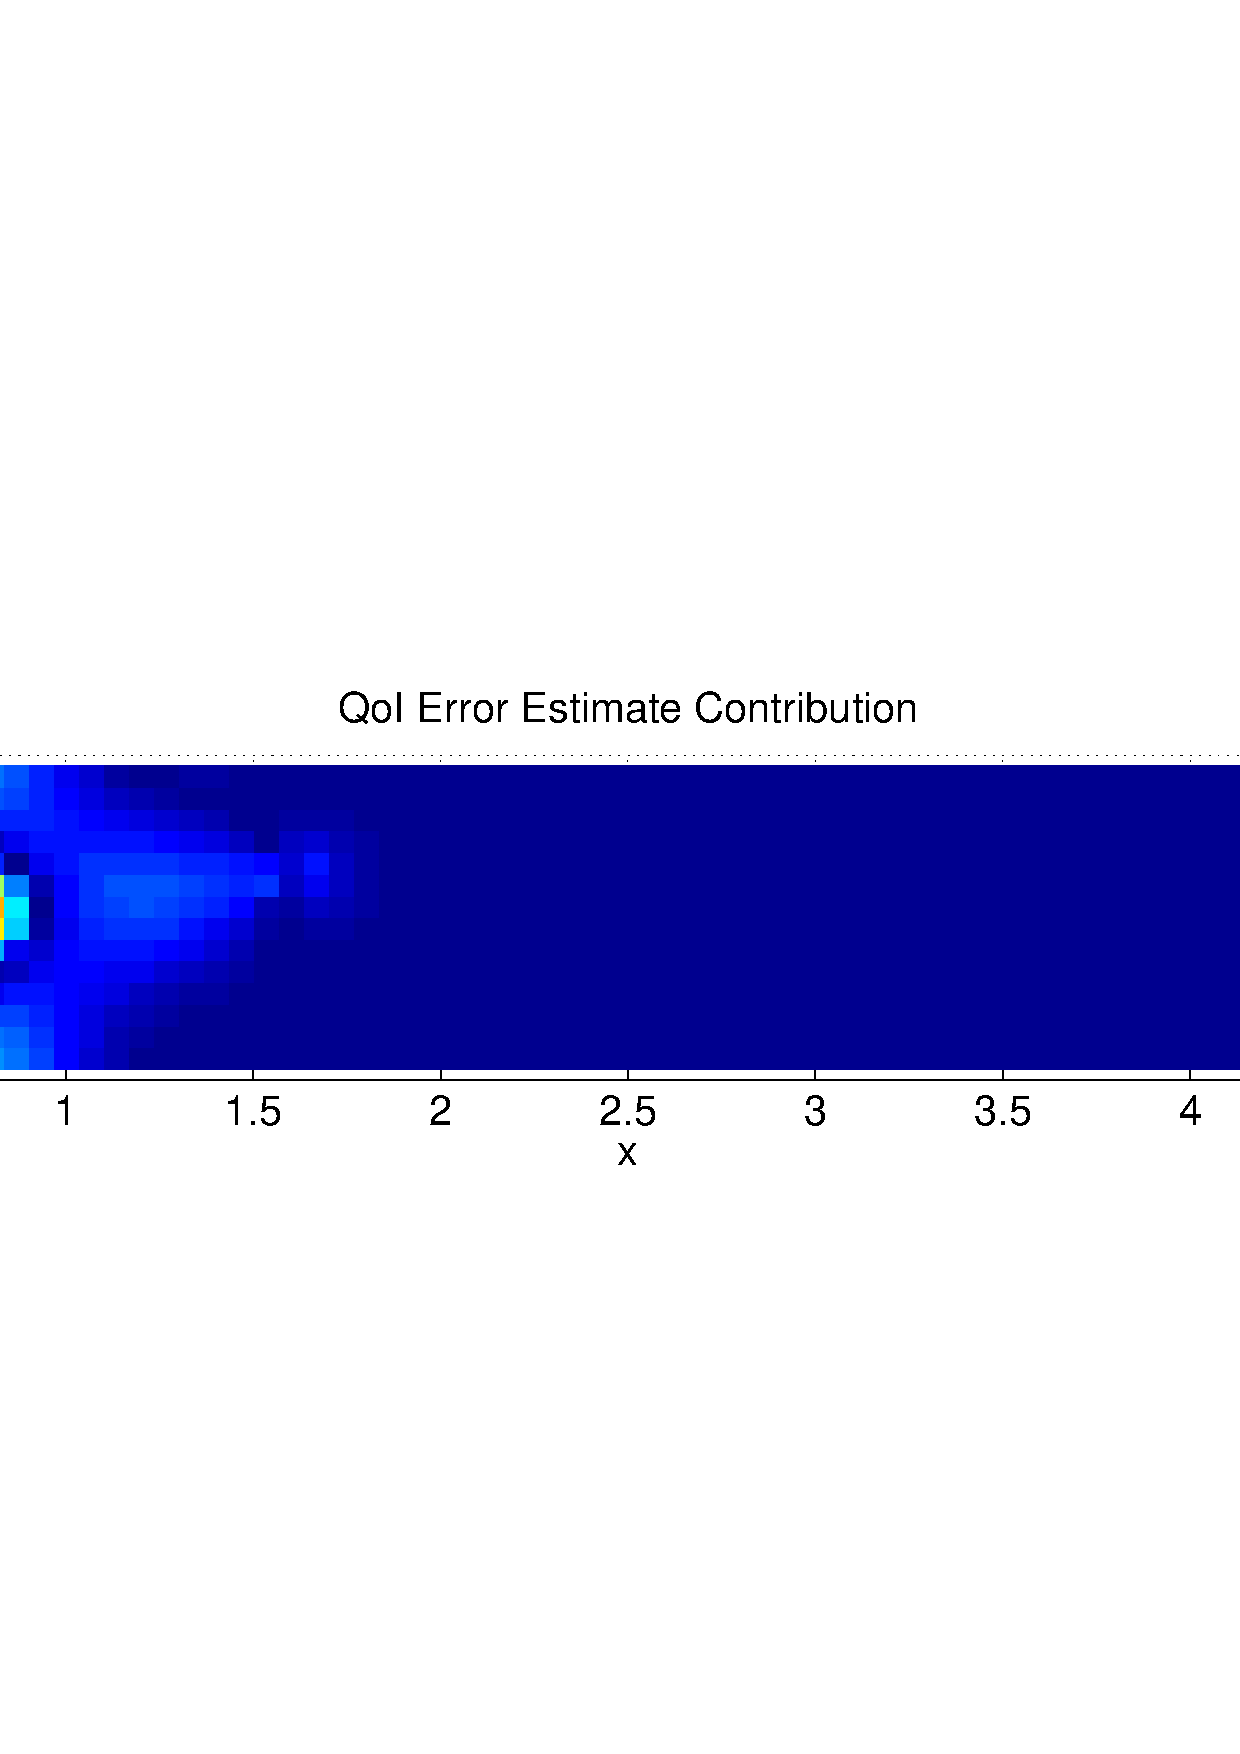
\includegraphics[width=0.49\textwidth]{baseSeries/err_breakdown_LF.png}
    \vspace{-0.5\baselineskip}
    \caption{MF$_0$ ($0\%$ HF)}
    \label{fig:baseRef0}
    \vspace{0.8\baselineskip}
  \end{subfigure}
	\begin{subfigure}[b]{\textwidth}
  \centering
    \includegraphics[width=0.48\textwidth]{baseSeries/cd_cdr_MF01_divvy.png}
    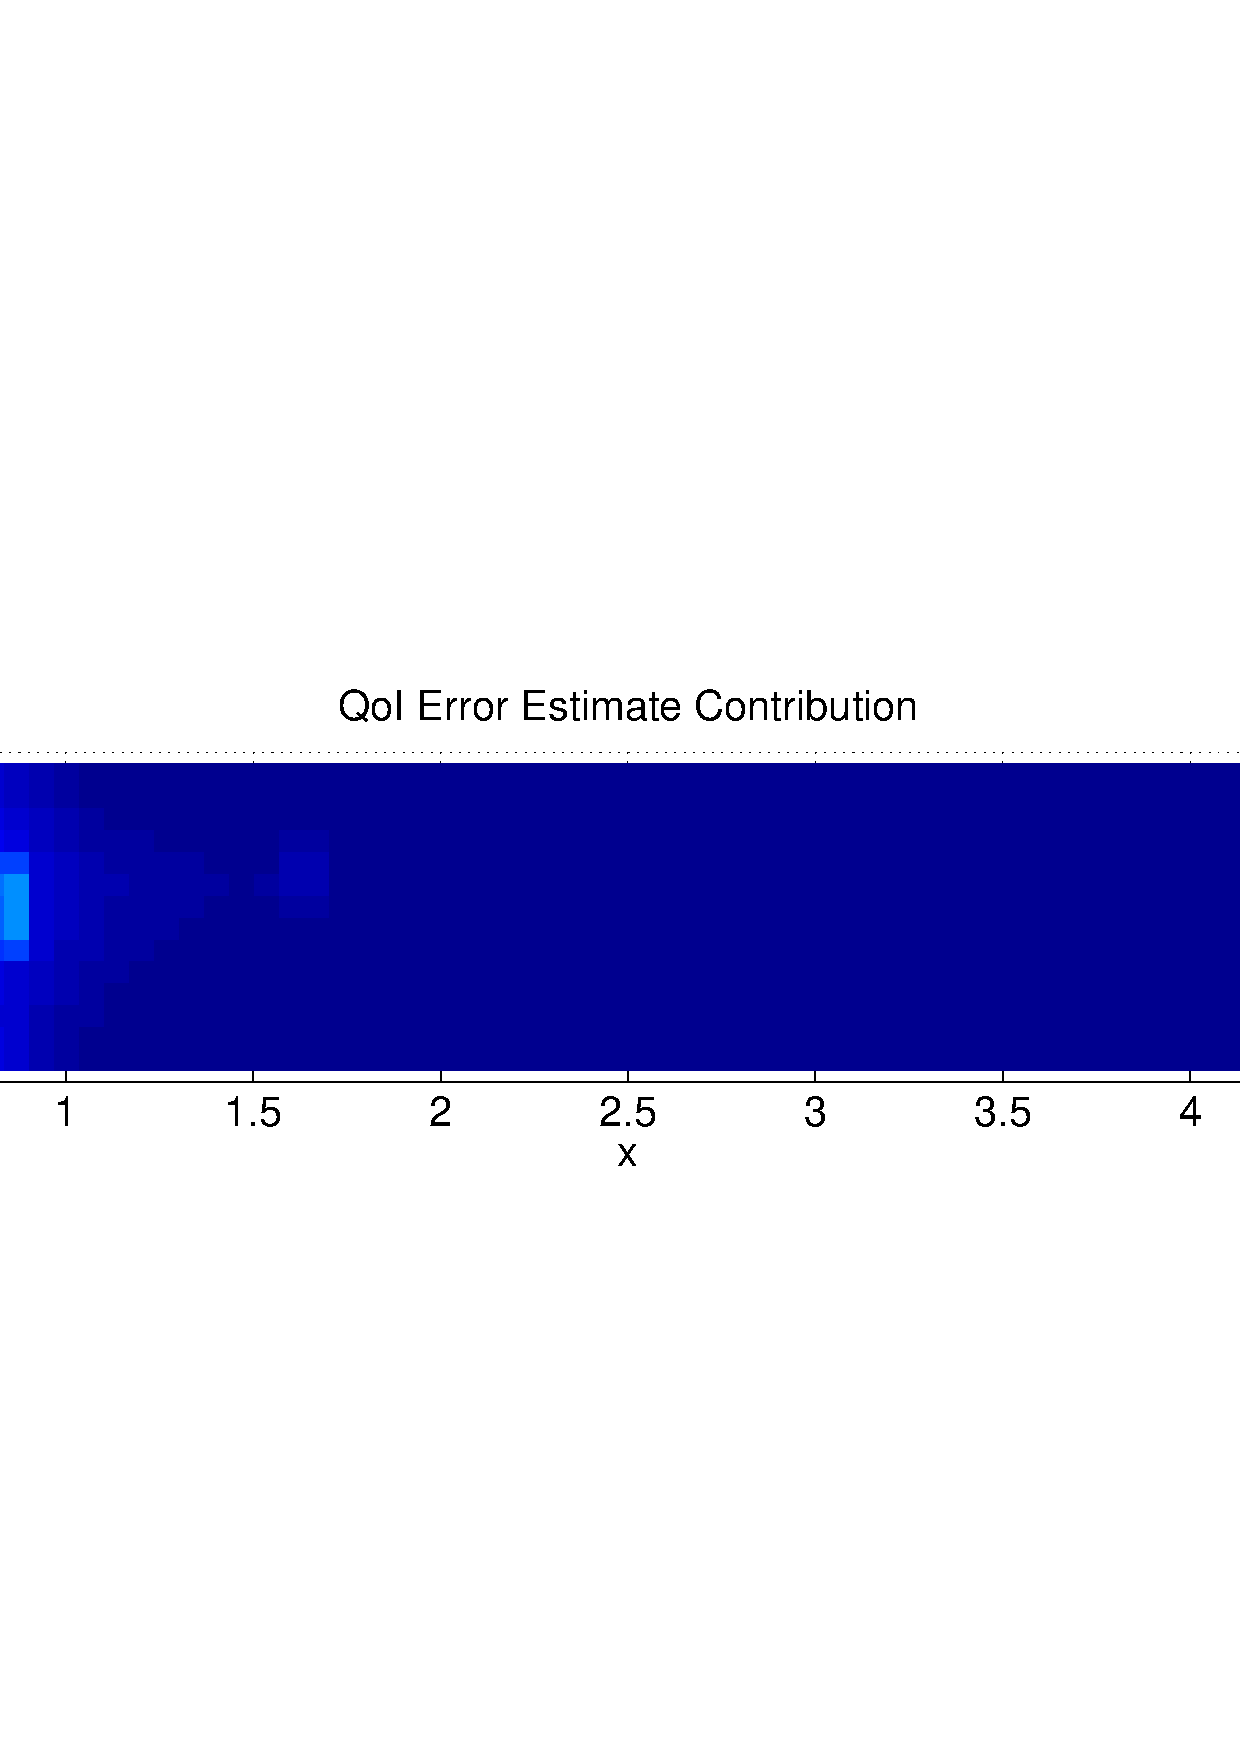
\includegraphics[width=0.49\textwidth]{baseSeries/err_breakdown_MF01.png}
    \vspace{-0.5\baselineskip}
    \caption{MF$_1$ ($5\%$ HF)}
    \vspace{0.8\baselineskip}
  \end{subfigure}
  \begin{subfigure}[b]{\textwidth}
  \centering
    \includegraphics[width=0.48\textwidth]{baseSeries/cd_cdr_MF02_divvy.png}
    \includegraphics[width=0.49\textwidth]{baseSeries/err_breakdown_MF02.png}
    \vspace{-0.5\baselineskip}
    \caption{MF$_2$ ($10\%$ HF)}
    \vspace{0.8\baselineskip}
  \end{subfigure}
\caption{Element-wise decomposition of error estimate (right) and domain division (left; low-fidelity convection-diffusion model used in red portion, high-fidelity convection-diffusion-reaction model used in blue portion) for mixed-fidelity models.}
\label{fig:baseRef}
\end{figure}
%
Note that since linear nodal basis elements are used, elements in regions where the high-fidelity model is already being used do not contribute to the error estimate, except some elements near the interface, whose basis function have support in both regions.

We see that model refinement is concentrated in the QoI region, and the data point closest to the QoI. In the first elemental decomposition of the error (Figure~\ref{fig:baseRef0}), the region where the elemental error is maximum is data point one. Since the constraining model is an elliptic PDE, with a weak convection, information flow is localized, and is weakly convected from left to right. Therefore, for the calculation of the QoI, it is most important to refine the region near data point one, and the QoI region. 
We also observe that the region near the data points downstream from the QoI are not refined as much as the region immediately adjacent to the QoI. This indicates that the information from these two data points is not significant for the estimation of the QoI. \red{We should say a bit more about the refinement region here, and implications for experimental design ?}. 

Figure~\ref{fig:baseErr} shows the true and estimated absolute relative errors in the QoI for the various mixed-fidelity models generated by algorithm~\ref{alg:refSeries}. It can be seen that the error estimates are close to the true error, and the error estimator has an effectivity index close to one. We also see that the QoI error of only $1\%$ is attained with a mixed-fidelity model where the high-fidelity model is used in only about $10\%$ of the domain.
%
\begin{figure}[h]
\centering
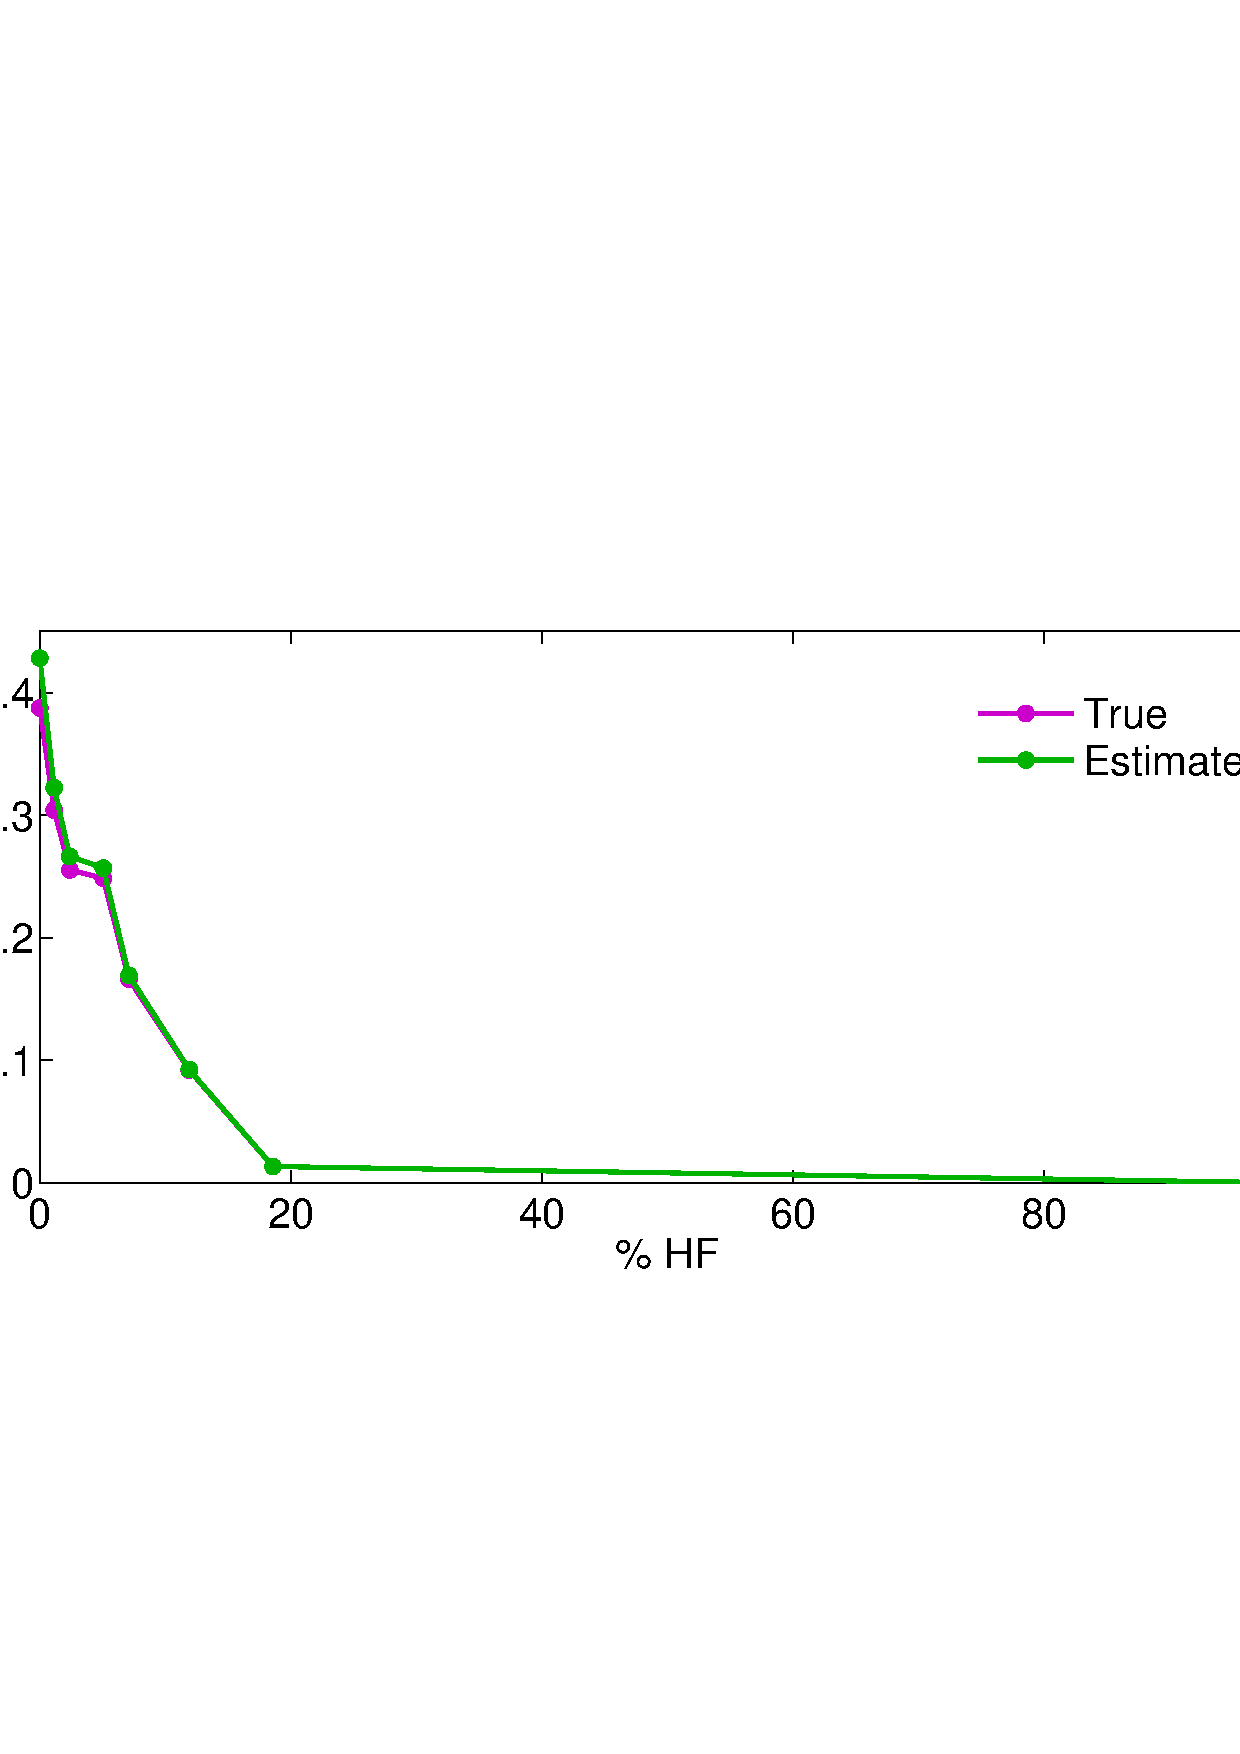
\includegraphics[width=0.8\textwidth]{baseSeries/err_est.pdf}
\caption{True and estimated absolute relative error in QoI, plotted as a function of the percentage area of the domain in which the high-fidelity convection-diffusion-reaction model is used.}
\label{fig:baseErr}
\end{figure}
%
\subsection{Constant vs Field Parameters}
%
\subsubsection{Problem Setup}
%
\subsubsection{Results}
%
\subsection{Convection-Diffusion(-Highly Nonlinear Reaction)}
%
\subsubsection{Results}
%
We consider the convection-diffusion-reaction term described in Section \ref{sec:cdvcdr}, with a reaction term $k_r=-616$ in the high-fidelity model. This reaction term is large enough that the Newton solver will not converge with a zero initial guess. We first solve the inverse problem with the low-fidelity model ($k_r=0$), and then use a simple continuation approach, using the solution at one value of $k_r$ as the initial guess for the next.\footnote{not arclength continuation, which is more difficult to implement, though libMesh appears to have a class for such continuation, which we can use if this seems like a viable direction} We increase the reaction term in increments of $\Delta k_r=100$, and halve the increment each time the step is too large (Newton solver does not converge at the next $k_r$ value). From $k_r=0$ to $k_r=-616$, this results in 9 continuation steps being taken.
%
\subsubsection{Computational Complexity}
%
We compare the complexity of algorithm~\ref{alg:refSeries} and the continuation method for the high fidelity problem, in the context of the analysis developed in section~\ref{sect:alg_complexity}. For the high fidelity problem, with  with 9 continuation steps, we have $\sum\limits_{i=1}^{C} K_i=30$. 
 
With Gaussian elimination chosen as the linear solver, this gives us $T < 3$, i.e.\ a budget of 2 adaptive steps. Using algorithm~\ref{alg:refSeries} with 2 refinement steps, and only $10\%$ of the domain refined to use the high-fidelity model, the estimated relative error is $<1\%$. Indeed, the ratio $\frac{C_{MF}}{C_{HF}}$ was $\frac{24}{30}$, indicating about $20\%$ reduction in computational cost, with the worst case linear solver used. 

In other words, on using algorithm~\ref{alg:refSeries} for a highly nonlinear problem, even with the worst case linear solver, one can get to $<1\%$ error in the QoI, with a $20\%$ reduction in computational cost, while avoiding any need for continuation to handle nonlinearities. 
